%----------------------------------------------------------------------------------------
%	PACKAGES AND THEMES
%----------------------------------------------------------------------------------------

\documentclass{beamer}

\mode<presentation> {

\usetheme{Madrid}

}


\usepackage{graphicx} % Allows including images
\usepackage{booktabs} % Allows the use of \toprule, \midrule and \bottomrule in tables

\usepackage[normalem]{ulem} % strike text
\usepackage{verbatim}

%%% Работа с русским языком
\usepackage[T2A]{fontenc}			% кодировка
\usepackage[utf8]{inputenc}			% кодировка исходного текста
%\usepackage[english]{babel}
\usepackage[english, russian]{babel}	% локализация и переносы


%%% Работа с картинками
\setlength\fboxsep{3pt} % Отступ рамки \fbox{} от рисунка
\setlength\fboxrule{1pt} % Толщина линий рамки \fbox{}
\usepackage{wrapfig} % Обтекание рисунков текстом

%%% Оформление стихов
\usepackage{verse}

\usepackage{ulem}

\AtBeginSection[]
{
  \begin{frame}
    \frametitle{Содержание}
    \tableofcontents[currentsection]
  \end{frame}
}


%----------------------------------------------------------------------------------------
%	TITLE PAGE
%----------------------------------------------------------------------------------------

\title[Занятие 2]{Формальный анализ стиха. Занятие 2} % The short title appears at the bottom of every slide, the full title is only on the title page

\author{Борис Орехов} % Your name
\institute[НИУ ВШЭ] % Your institution as it will appear on the bottom of every slide, may be shorthand to save space
{
НИУ Высшая школа экономики \\ % Your institution for the title page
\medskip
\textit{nevmenandr@gmail.com} % Your email address
}
\date{15 сентября 2015} % Date, can be changed to a custom date

\begin{document}

\begin{frame}
\titlepage % Print the title page as the first slide
\end{frame}



\begin{frame}
\frametitle{Содержание}  % Table of contents slide, comment this block out to remove it
\tableofcontents % Throughout your presentation, if you choose to use \section{} and \subsection{} commands, these will automatically be printed on this slide as an overview of your presentation
\end{frame}

%----------------------------------------------------------------------------------------
%	PRESENTATION SLIDES
%----------------------------------------------------------------------------------------



%------------------------------------------------
\section{Анкеты}\label{sec:ank} % Sections can be created in order to organize your presentation into discrete blocks, all sections and subsections are automatically printed in the table of contents as an overview of the talk
%------------------------------------------------

%\subsection{Зачем пишут стихи}\label{sec:why} % A subsection can be created just before a set of slides with a common theme to further break down your presentation into chunks

%------------------------------------------------

\begin{frame}
\frametitle{Опрос про знакомство с поэтами}

\begin{itemize}
\item проводится уже~третий раз;
\item даёт возможность оценить <<масштабы бедствия>>;
\item по~итогам опроса проводится кластеризация (разбиение на~группы по~сходству) и~строится дендрограмма;
\item дендрограмма позволяет оценить, какие поэты схожи между собой по~восприятию;
\item изначально это не картина того, кого знают и~кого не~знают; это картина того, про~кого респонденты отвечают одинаково;
\item если два~респондента хорошо знают и~Ахматову, и~Цветаеву, то~те~попадут в~один кластер;
\item если один респондент знает Заболоцкого, но~не~знает Тарковского, а~другой наоборот, то~поэты окажутся далеко друг от~друга на~графике;
\item не~формальный анализ стиха, но~формальный анализ восприятия.
\end{itemize}

\end{frame}

%------------------------------------------------

\begin{frame}
\frametitle{Получается матрица}

\begin{table}[]
\centering
\caption{Матрица ответов}
\label{my-table}
\begin{tabular}{lllll}
Георгий Адамович     & 0 & 0 & 0 & 2 \\
Иннокентий Анненский & 1 & 0 & 0 & 3 \\
Анна Ахматова        & 3 & 2 & 4 & 4 \\
Евгений Баратынский  & 1 & 1 & 2 & 2
\end{tabular}
\end{table}


\end{frame}

%------------------------------------------------

\begin{frame}
\frametitle{Дендрограмма ответов студентов, поступивших в~2011}
\begin{center}
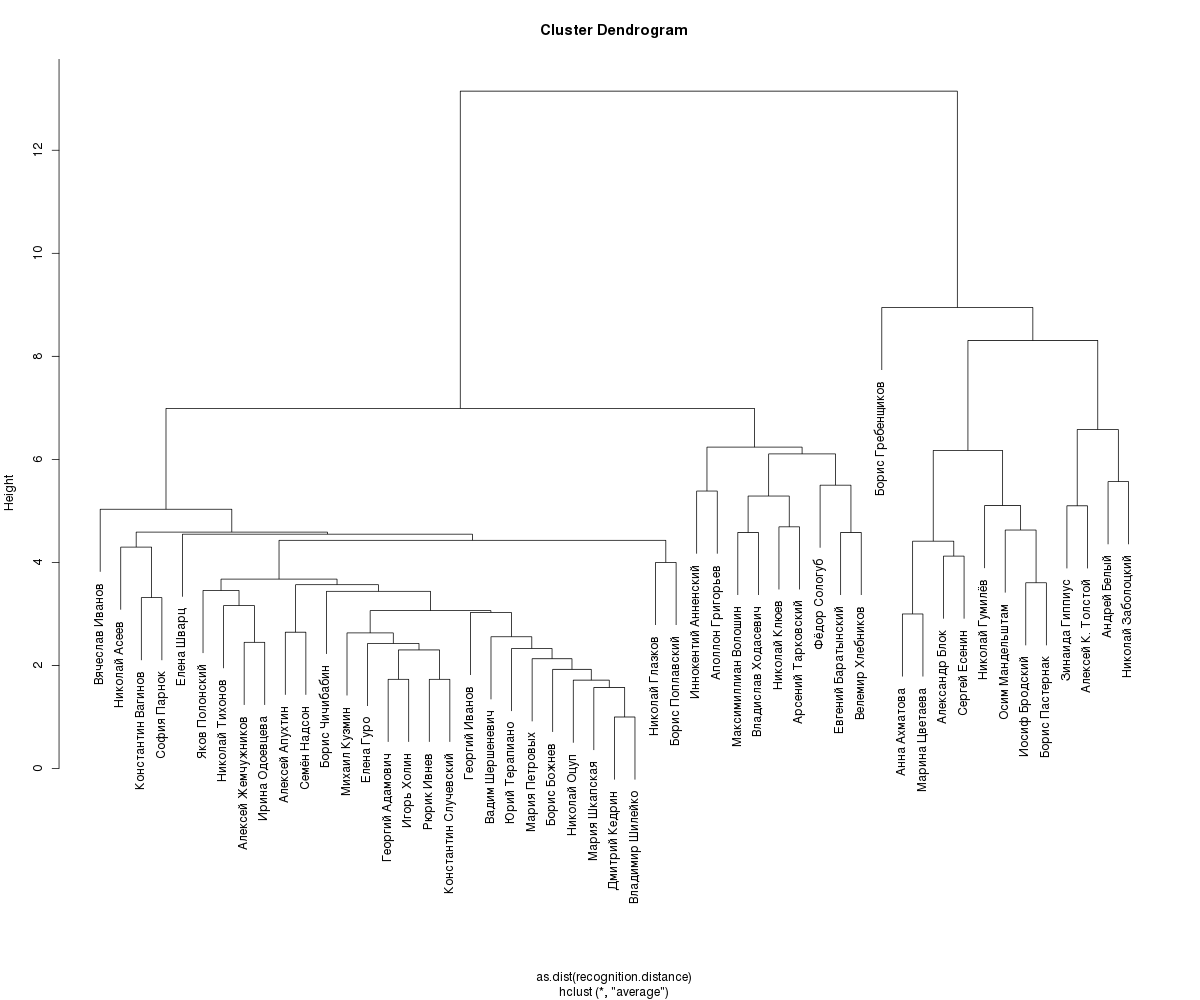
\includegraphics[width=0.85\textwidth]{clust1.png}
\end{center}
\end{frame}

%------------------------------------------------

\begin{frame}
\frametitle{Дендрограмма ответов студентов, поступивших в~2012}
\begin{center}
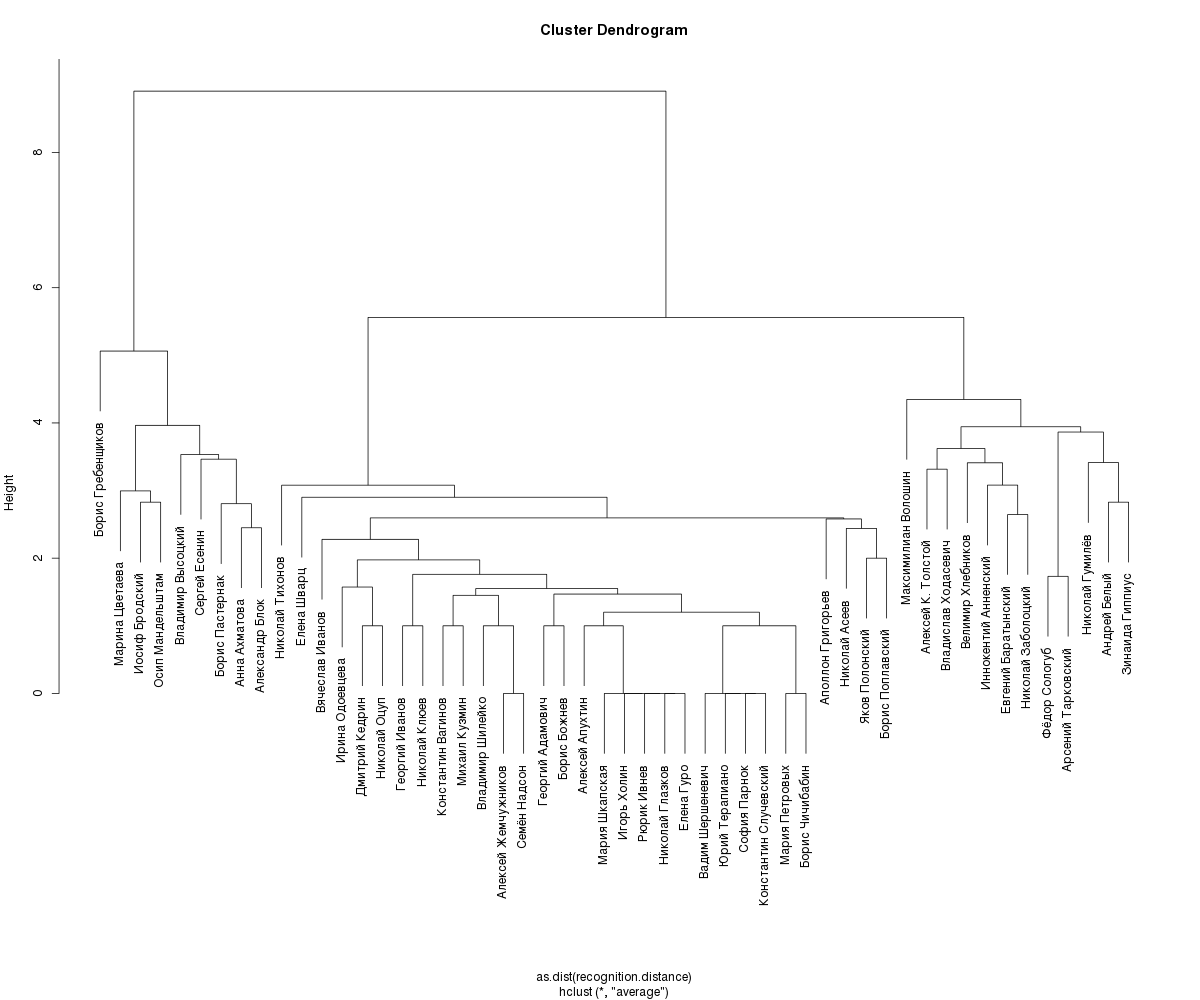
\includegraphics[width=0.85\textwidth]{clust2.png}
\end{center}
\end{frame}

%------------------------------------------------

\begin{frame}
\frametitle{Ваши ответы}
\begin{center}
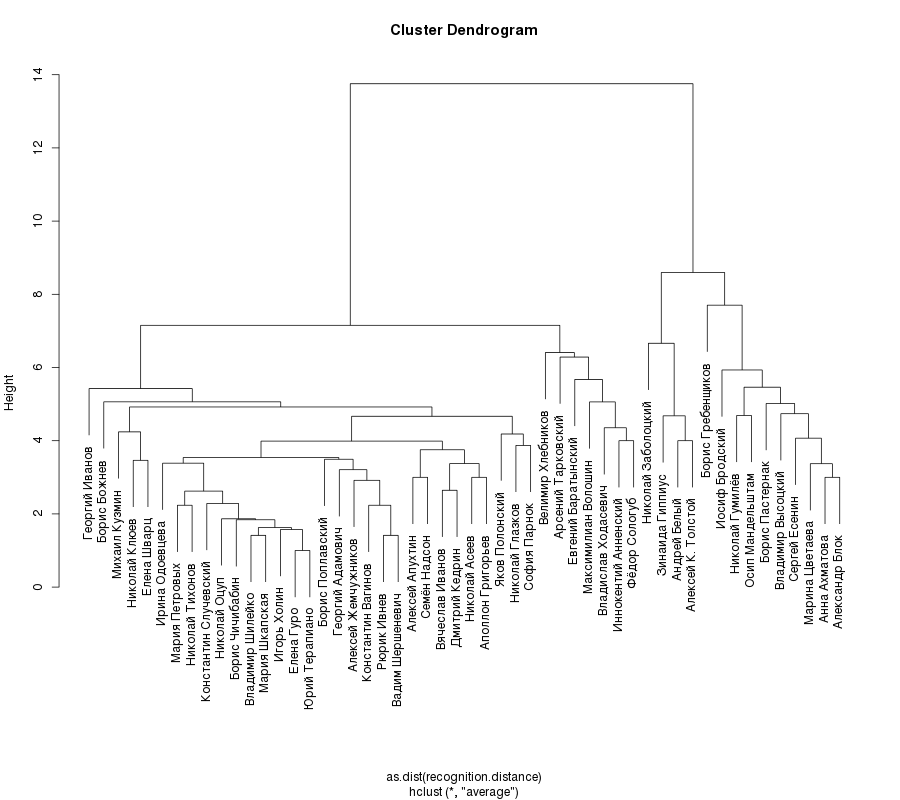
\includegraphics[width=0.8\textwidth]{clust3.png}
\end{center}
\end{frame}

%------------------------------------------------

\begin{frame}
\frametitle{Как повысить свой уровень?}

\begin{center}
{\LARGE http://poetae.narod.ru/}
\end{center}

Поэтическая антология, составленная Д.",В.",Сичинавой.

\end{frame}

%------------------------------------------------

\section{Структура курса}\label{sec:struct}

%------------------------------------------------

%------------------------------------------------

\begin{frame}
\frametitle{Структура курса}
\begin{itemize}
\item Стих и проза;
\item Метрика;
\begin{itemize}
\item Системы стихосложения;
\item Русская силлабика;
\item Реформа стиха и~силлабо"=тоника;
\item Пеоны, гиперпеоны;
\item Разрешенные преобразования внутри силлабо"=тонической модели; метрическая неоднозначность;
\item Гетерометрия, разностопный стих, каталектика;
\item Неклассические размеры;
\end{itemize}
\item Поэтика;
\begin{itemize}
\item Фоника стиха;
\item Грамматика;
\begin{itemize}
\item Поэтическая морфология;
\item Поэтический синтаксис;
\item Лингвистика стиха;
\end{itemize}
\item Лексика и~семантика стиха, тропы;
\item Текстология и установление авторства по~формальным параметрам.
\end{itemize}

\end{itemize}

\end{frame}

% --------------------------------

\begin{frame}
\frametitle{Что читать?}
Литература общего назначения
\begin{itemize}
\item Гаспаров",М.",Л. Очерк истории русского стиха. М.: Фортуна Лимитед, 2003.
\item Гаспаров",М.",Л. Очерк истории европейского стиха. М.: Фортуна Лимитед, 2003.
\item Гаспаров",М.",Л. Русски\sout{е}й стих\sout{и} начала XX~века в~комментариях. М.: КДУ, 2004.
\item Ярхо",Б.",И. Методология точного литературоведения. Избранные труды по~теории литературы. М.: Языки славянской культуры, 2006.
\item Лотман",Ю.",М. Анализ поэтического текста.
\item Томашевский",Б.",В. Теория литературы. Поэтика.
\end{itemize}
\end{frame}

%------------------------------------------------

% --------------------------------

\begin{frame}
\frametitle{Что читать?}
Литература специального назначения
\begin{itemize}
\item Леви"=Стросс",К., Якобсон",Р. <<Кошки>> Шарля Бодлера.
\item Шапир",М.",И. Гекзаметр и пентаметр в поэзии Катенина.
\item Гаспаров",М.",Л., Скулачева",Т.",В. Статьи о~лингвистике стиха.
\item Хетсо",Г. Лексика стихотворений Лермонтова. Опыт количественного описания.
\end{itemize}
\end{frame}

\section{Анализ стиха: формальный и неформальный}\label{sec:formal}

%------------------------------------------------

\begin{frame}
\frametitle{Как анализируют стих неформально?}
\begin{itemize}
\item социологизм; 
\item биография поэта; исторический контекст: \\
\begin{flushleft}
Стихотворение Тютчева <<Цицерон>>: отголосок июльской революции 1830~года?
\end{flushleft}
\item интертекстуальные параллели: \\
\begin{flushleft}
Прощай~же, книга! Для~видений отсрочки смертной тоже нет. С~колен поднимется Евгений, но~удаляется поэт. И~все~же слух не~может сразу расстаться с~музыкой, рассказу дать замереть\ldots судьба сама еще звенит, и~для~ума внимательного нет границы там, где~поставил точку~я: продленный призрак бытия синеет за~чертой страницы, как завтрашние облака, и~не~кончается строка.
\end{flushleft}

В.",В.",Набоков <<Дар>>
1938

\end{itemize}

\end{frame}

%------------------------------------------------
%
\begin{frame}
\frametitle{Формализм 1930"=х годов}

\begin{itemize}
\item Реакция на~биографизм и~социологизм
\item Понятие приёма и~минус"=приёма
\item Б.",В.",Томашевский, Ю.",Н.",Тынянов, В.",Я.",Пропп, Б.",М.",Эйхенбаум, Б.",Я.",Бухштаб
\end{itemize}

\end{frame}

%------------------------------------------------

\section{Стих и~проза: пограничные случаи}\label{sec:limit}

%------------------------------------------------

\begin{frame}
\frametitle{Вопросы с~прошлого занятия}

\begin{itemize}
\item Чем профессиональная поэзия отличается от~непрофессиональной?
\item Что такое теснота стихового ряда?
\item Чем стихи отличаются от~прозы?
\end{itemize}

\end{frame}

%------------------------------------------------

\begin{frame}
\frametitle{Стихи?}

\begin{verse}
Ассорти рыбное\\
Тарталетки с~красной икрой\\
Закуска по"=русски\\
Куриный рулет\\
Бастурма	\\
Ассорти мясное\\	
Язык отварной\\
Ассорти баклажаны\\
Соленья по"=домашнему
\end{verse}

\end{frame}



%------------------------------------------------

\begin{frame}
\frametitle{Стих и~проза: пограничные случаи}

\begin{center}
\textbf{Большая элегия Анатолию Чубайсу}
\end{center}

\begin{flushleft}
Чубайс уснул, уснуло все вокруг. Его~враги невольно оробели: под~шум листвы, под~вой рублевских вьюг он~крепко спит в~хрустальной колыбели. Он~помещен в~особый мавзолей, лишь через пару лет назначен вынос\ldots Пока не~спал он "--- было веселей, но~вот уснул, и~все остановилось. Морфей его в~объятьях приласкал. Горит ночник, включенный для~уюта. Вертелось все, покуда он~не~спал: росла национальная валюта, дошли до~пика цены на~сырье, качалась нефть "--- хоть~пей, хоть~умывайся\ldots Порою омрачала бытие коррупция, но~супротив нее боролись все, включая и~Чубайса. Крутились деньги. Делались дела. Простой народ стонал от~монополий. Короче, при~Чубайсе жизнь была, но~хочет спать железный Анатолий. <\ldots>
\end{flushleft}

Дмитрий Быков\\
2008
\end{frame}

%------------------------------------------------

\begin{frame}
\frametitle{Иосиф Бродский <<Большая элегия Джону Донну>>}

\begin{verse}
Джон Донн уснул, уснуло все~вокруг.\\
Уснули стены, пол, постель, картины,\\
уснули стол, ковры, засовы, крюк,\\
весь гардероб, буфет, свеча, гардины.\\
Уснуло все. Бутыль, стакан, тазы,\\
хлеб, хлебный нож, фарфор, хрусталь, посуда,\\
ночник, белье, шкафы, стекло, часы,\\
ступеньки лестниц, двери. Ночь повсюду.\\
Повсюду ночь: в~углах, в~глазах, в~белье,\\
среди бумаг, в~столе, в~готовой речи,\\
в~ее словах, в~дровах, в~щипцах, в~угле\\
остывшего камина, в~каждой вещи. <\ldots> 
\end{verse}

1963

\end{frame}

%------------------------------------------------

\begin{frame}
\frametitle{Мнимая проза}
\begin{flushleft}
Петербуржанке и~северянке люб мне ветер с~гривой седой, тот, что~узкое горло Фонтанки заливает невской водой.\\
Знаю "--- будут любить мои дети невский седобородый вал, оттого, что~был западный ветер, когда ты~меня целовал.
\end{flushleft}

1922
\begin{flushleft}
\footnotesize{Мария Михайловна Шкапская
(3~октября 1891, Петербург\,--\,7~сентября 1952, Москва)\\
Выпустила 6~маленьких стихотворных книжек в~1921\,--\,1925 гг.; в~них говорилось о~судьбе и~назначении женщины, которая, рожая детей, передает им~неумирающую наследственность единого человечества. Одобрявшие критики называли ее~стихи «женскими», суровые "--- «гинекологическими». Потом работала журналисткой. \\ 

Гаспаров «Русский стих начала XX~века в~комментариях»}
\end{flushleft}

\end{frame}

%------------------------------------------------

\begin{frame}
\frametitle{Рифмованная проза}

\begin{flushleft}
Мы услышали его во~всей неискаженной ясности 
его: был~подобен парению раненой птицы, был~снежного сверкающего цвета, \alert{пел} 
голос \alert{бел}, \alert{бел} голос \alert{был}, \alert{плыл} голос, голос плыл и~\alert{таял}, был голос \alert{тал}. Он~пробивался сквозь все, все презирая, он~возрастал и падал, дабы возрасти.
\end{flushleft}

Саша Соколов «Школа для дураков»\\
1973

\end{frame}

%------------------------------------------------


\begin{frame}
\frametitle{Ритмизованная проза}

\begin{flushleft}
Что есть Русская Империя наша?\\
Русская Империя наша есть географическое единство, что значит: часть известной планеты. И~Русская Империя заключает: в"=-первых "--- великую, малую, белую и~червонную Русь; во"=вторых "--- грузинское, польское, казанское и~астраханское царство; в"=третьих, она заключает\ldots Но "--- прочая, прочая, прочая. \\
Русская Империя наша состоит из~множества городов: столичных, губернских, уездных, заштатных; и~далее: "--- из первопрестольного града и~матери градов русских.
Град первопрестольный "--- Москва; и~мать градов русских есть Киев.
\end{flushleft}

Андрей Белый <<Петербург>>\\
1912\,--\,1913

\end{frame}

%------------------------------------------------
%
\begin{frame}
\frametitle{Ритмизованная проза}

\begin{flushleft}
Высоко в горы вполз Уж и лег там в сыром ущелье, свернувшись в узел и глядя в море.\\
Высоко в небе сияло солнце, а горы зноем дышали в небо, и бились волны внизу о камень...\\
А по ущелью, во тьме и брызгах, поток стремился навстречу морю, гремя камнями...\\
Весь в белой пене, седой и сильный, он резал гору и падал в море, сердито воя.\\
Вдруг в то ущелье, где Уж свернулся, пал с неба Сокол с разбитой грудью, в крови на перьях...\\
С коротким криком он пал на землю и бился грудью в бессильном гневе о твердый камень...
\end{flushleft}

Максим Горький «Песня о~Соколе»\\
1895

\end{frame}
%
%%------------------------------------------------
%
\begin{frame}
\frametitle{Стихотворение в прозе}

\begin{flushleft}
Я~шел по~широкому полю, один.\\
И~вдруг мне почудились легкие, осторожные шаги за~моей спиною\ldots Кто"=то шел по~моему следу.\\
Я~оглянулся "--- и~увидал маленькую, сгорбленную старушку, всю закутанную в~серые лохмотья. Лицо старушки одно виднелось из"=под~них: желтое, морщинистое, востроносое, беззубое лицо.
Я~подошел к~ней\ldots Она~остановилась.\\
"--* Кто ты? Чего тебе нужно? Ты~нищая? Ждешь милостыни?\\
Старушка не~отвечала. Я~наклонился к~ней и~заметил, что оба глаза у~ней были застланы полупрозрачной, беловатой перепонкой, или~плевой, какая бывает у~иных птиц: они~защищают ею~свои глаза от~слишком яркого света.\\
Но~у~старушки та~плева не~двигалась и не открывала зениц\ldots из~чего я~заключил, что она слепая. <\ldots>
\end{flushleft}

И.",С.",Тургенев «Старуха»\\
1878\,--\,1882

\end{frame}

%%------------------------------------------------
%
\begin{frame}
\frametitle{Анжанбеман, анжамбман, анжанбеман, анжамбаман, энжанбеман\ldots}

enjambement

\begin{verse}
Ниоткуда с любовью, надцатого мартобря,\\
дорогой, уважаемый, милая, но \alert{неважно}\\
\alert{даже кто}, ибо черт лица, \alert{говоря}\\
\alert{откровенно}, не вспомнить, уже не ваш, \alert{но}\\
\alert{и ничей} верный друг вас приветствует \alert{с одного}\\
\alert{из пяти} континентов, держащегося на ковбоях;\\
я любил тебя больше, чем ангелов и самого,\\
и поэтому дальше теперь от тебя, чем от них обоих...
\end{verse}

И.",Бродский\\
1976

\end{frame}

%------------------------------------------------

\begin{frame}
\Huge{\centerline{продолжение следует}}
\end{frame}

%----------------------------------------------------------------------------------------

\end{document}